\documentclass[font=10pt]{article}
\usepackage[left=1cm,right=1cm,top=1cm,bottom=1cm]{geometry}
\usepackage{graphicx}
\usepackage{float}
%\setcounter{tocdepth}{4}
\graphicspath{ {./images/} }
\begin{document}

  \begin{titlepage}
    \centering
    \title{\textbf{INFO3406 Assignment Stage 2}}
    \author{
      Nick Zhou 460363707\\
      Linzi Zhu 460381996
    }
    \date{October 2018}
    \maketitle
    
\includegraphics[width=5cm]{usyd}
  \end{titlepage}

  \begin{tableofcontents}
    \tableofcontents
    \pagebreak
  \end{tableofcontents}

  \section{Section 1: Setup}
    \subsection{Research Questions and Hypothesis}
    % State your research question(s). State null and alternative hypotheses
      \subsubsection{Research Questions}

	In any project, choosing a title can be one of the most difficult aspects, as the title is often the first thing any member of your audience knows about the material. In order to aid people in choosing better project titles, we aim to find if there was a way to mathematically model the impact that a movie title has on a film's box-office success.

      Specfically, the research questions we will attempt to answer is:
      \begin{enumerate}
        \item Is there a link between the emotional response a movie’s title evokes (sight unseen) and the movies eventual gross revenue?
        \item Using these models, can we train a predictor to assess the value of a title for any given movie?
      \end{enumerate}

      \subsubsection{Hypotheses}

      \underline{Hypotheses}
      \begin{itemize}
        \item H0 (the null Hypothesis): The emotional impact of the lexicon used in movie titles \textit{does not have a statistically significant effect} on the box-office performance of a movie in gross revenue.
        \item H1 (the alternative Hypothesis):The emotional impact of the lexicon used in movie titles in movie does \textit{has a statistically significant effect} on the box-office performance of a movie.
      \end{itemize}

    \subsection{Reliability}
    % Describe how you will quantify reliability e.g. significance testing, confidence intervals. If appropriate, describe how you will measure effectiveness e.g. regression r-square, clustering V-measure, classification f1-score.
	As we intend to use a multiple linear regression predictor, validity and effectiveness will be measured through the following metrics.
	\newline
	\textbf{Validity}
	 \begin{itemize}
        \item \underline{Linear Relationship}: We assume that there exists a linear relationship between the dependent variable and the independent variables. We will determine if such a relationship exists through scatter-plot analysis and covariance analysis.
	 \item \underline{Multivariate Normality}: We assume that the residuals are normally distributed. We will check this using a predicted vs residual scatterplot post-regression.
	 \item \underline{No Multicolinearlity}: We assume that the independent variables are not too highly correlated. We will test this assumption using Variance Inflation Factor (VIF) values.
	\item \underline{Homoscedasticity}: We assume that the variance of error terms are similar across the values of the independent variables.  A plot of standardized residuals versus predicted values can show whether points are equally distributed across all values of the independent variables.
	\item \underline{Goodness of Fit} We use the adjusted $R^{2}$ coefficient of determination to determine how close our model fits the actual dataset, while avoiding the issue of the $R^{2}$ increasing due to the additional independent variables.
	\
      \end{itemize}
	\textbf{Effectiveness}
	\begin{itemize}
	\item \underline{Cross Validation} Finally, to test the effectiveness of our model, we will use cross validation and the root mean squared prediction error to determine how well our model predicts data not present in the training set.
	\end{itemize}


    \subsection{Dataset}
    % Identify datasets and the data you derived from them
    For this dataset we combined 2 larger datasets, while trimming some extraneous information not relevant to this report. A 2011 report from the National Research Council Canada on Word-Emotion Association Lexicon - acquired from https://saifmohammad.com/WebPages/NRC-Emotion-Lexicon.htm, and the IMDB5000 movie dataset, listing a huge amount of metadata related to 5000 select movies - acquired from https://github.com/Godoy/imdb-5000-movie-dataset
    \newline \newline
    The Word-Emotion Association Lexicon was originally compiled by asking volunteers on Amazon's Mechanical Turk to rate a series of words, the total of which were analysed and compiled into the report by the NRC. In particular, we used the word to Valence, Arousal and Dominance report, which takes a large number of English unigrams and assigns to each a value from 0 to 1 for valence, arousal and dominance. In order -

    \begin{itemize}
        \item Valence (sometimes known as pleasure) measures how pleasant or unpleasant one feels about something. For instance both anger and fear are unpleasant emotions, and both score on the displeasure side. However joy is a pleasant emotion.
        \item Arousal measures how energized or soporific one feels. It is not the intensity of the emotion -- for grief and depression can be low arousal intense feelings. While both anger and rage are unpleasant emotions, rage has a higher intensity or a higher arousal state. However boredom, which is also an unpleasant state, has a low arousal value.
        \item Dominance represents the controlling and dominant versus controlled or submissive one feels. For instance while both fear and anger are unpleasant emotions, anger is a dominant emotion, while fear is a submissive emotion
    \end{itemize}

    The IMDB5000 is essentially a scrape of the IMDB database, the stats for which are all user compiled, like Wikipedia.
    \newline \newline
    In our report, we take a combination of these statistics. Firstly, the titles of the films in question, stored as strings. Then the gross revenue of the film as described my IMDB, stored as an integer. Finally, we took an average of each of the valence, arousal and dominance values of each word in the corresponding titles, represented as a real number from 0-1.
    \newline \newline
    %\heading{cleaning}

   Using a specific SQL query (provided in the Stage 1 code report) we muxed the data, producing a list of 3460 movie titles, along with their gross revenue and an average of the valence, arousal and dominance of every non-particle english word in their titles. This was the final CSV file for use in this analysis.

Some histograms of this dataset are provided below

\begin{center}
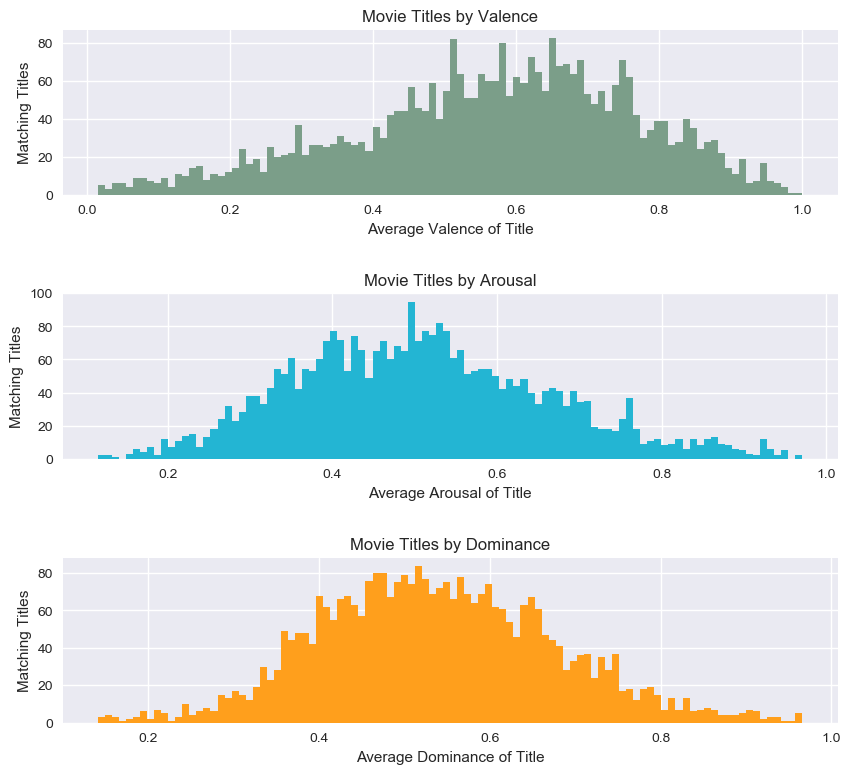
\includegraphics[width=15cm]{Movie_titles_by_vad.png}
\end{center}

  \section{Section 2: Approach}
 \begin{enumerate}
	\item   First, we worked to determine whether the assumptions held true in order to produce a valid linear regression model.
        \item \underline{Linear Relationship}: We performed both scatter-plot analysis and covariant analysis, using the Pearson Correlation coefficient, with 2-tailed significance tests, to determine the existence of a linear relationship.
	\item \underline {Split and Regression}As the next 4 tests require us to perform the regression, we split the dataset into 70\% training and 30\% testing samples and run the ordinary least squares linear regression.
	 \item \underline{Multivariate Normality}: We check the predicted vs residual scatterplot to determine multivariate normality.
	 \item \underline{No Multicolinearlity}: We will test this assumption using Variance Inflation Factor (VIF) values.
	\item \underline{Homoscedasticity}: We check the plot of standardized residuals versus predicted values to determine whether points are equally distributed across all values of the independent variables.
	\item \underline{Goodness of Fit} We use the adjusted $R^{2}$ coefficient of determination to determine how close our model fits the actual dataset.
	\item \underline{Cross Validation} We use our test sample to to check how closely the new data aligns to the line produced.
      \end{enumerate}
  \section{Section 3: Results}
The tests for linear relationship reveal something surprising. There exists a very weak linear relationship between every predictor variable and the gross box office perfomance. Both the scatterplot, a scatterplot using the square root of the gross variable (rtgross, created in order to normalise the extremely left skewed distribution, which makes the plot hard to examine) and the covariate analysis all show that (with a significance level of 0.05), there does not exist a statistically significant relationship between the dependants (valence, arousal and dominance) and the independant variable (gross).
\newline
\begin{center}
	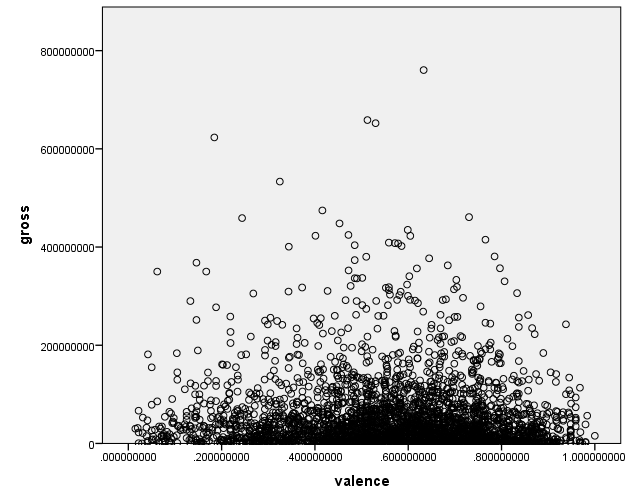
\includegraphics[width=10cm]{grosstovalence.png}
\newline
 	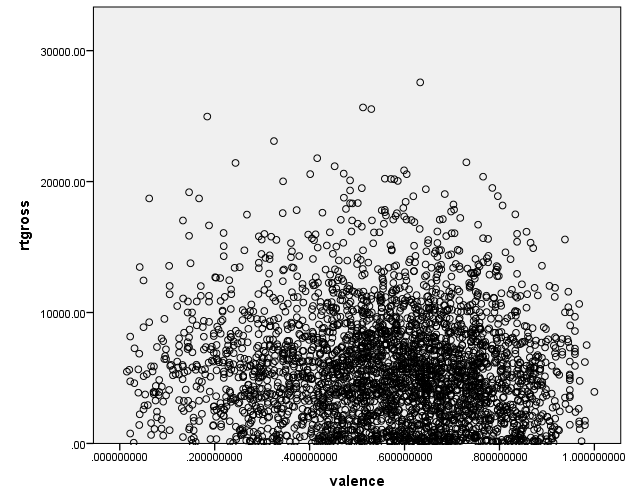
\includegraphics[width=10cm]{rtgrosstovalence.png}
\newline
	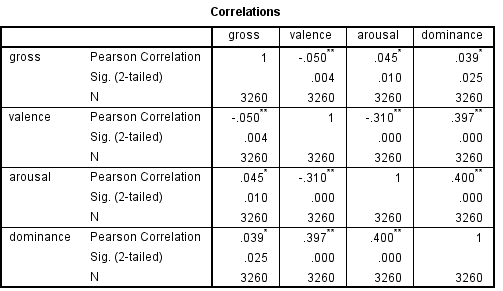
\includegraphics[width = 10cm]{correlations}
\end{center}

However, further testing proves that there does not exist a non-linear curve in the data, as all curves simply flatten out and become linear across the very low values of gross, as the distribution is extremely left-skewed, as demonstrated in the curve estimation graphs below.

With that in mind, we will continue with the linear regression analysis.

\begin{center}
	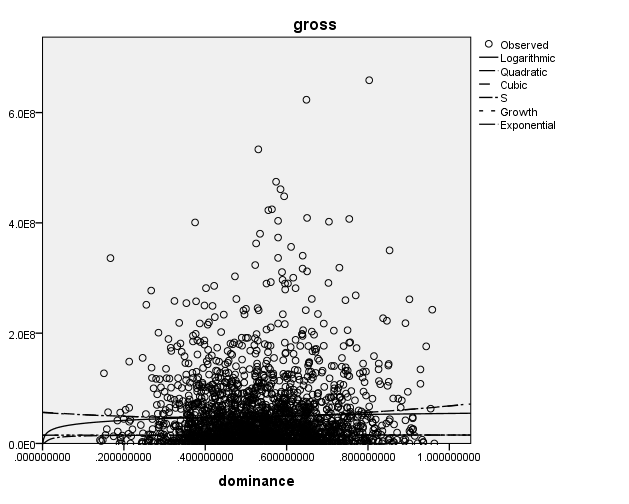
\includegraphics[width=12cm]{curve_estimation}
	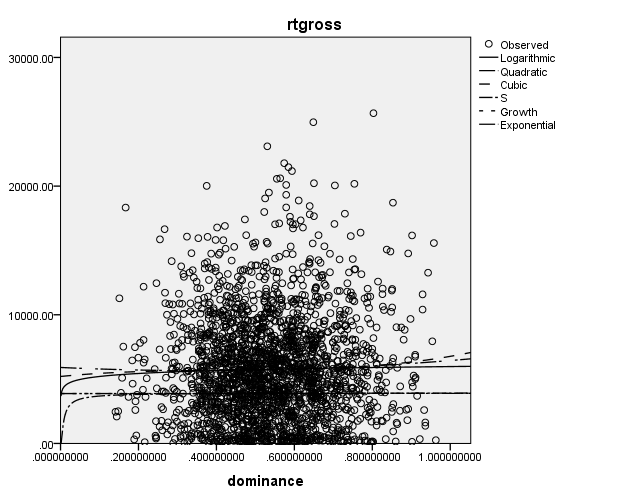
\includegraphics[width=12cm]{rtgross_curve_estimation}
\end{center}

Using the QQ plots we can see that, while all the 3 independent variables are slightly fat tailed, they are all quite normally distributed, meaning we have multivariate normality.

\begin{center}
	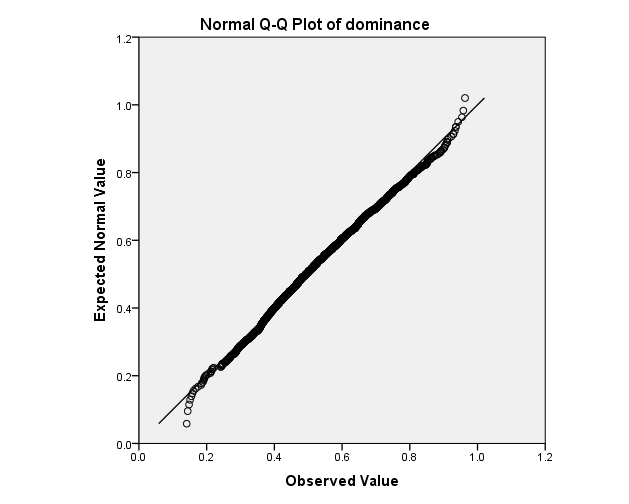
\includegraphics[width=10cm]{dominanceqq}
\end{center}

Next, the predicted vs residual scatterplot indicates that our results are nowhere near homoscedatic, showing massive differences in variability.

\begin{center}
	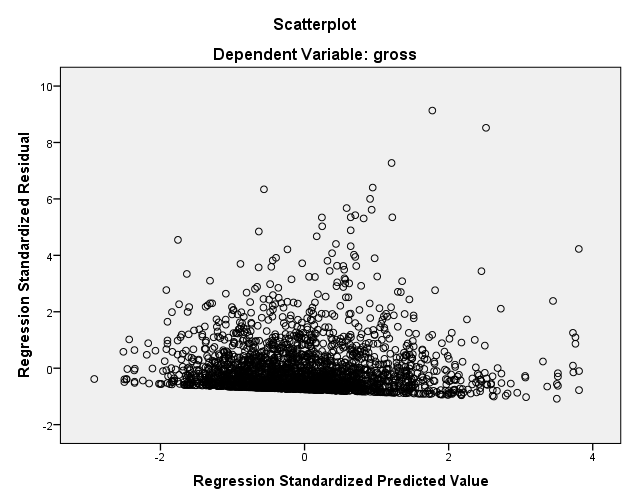
\includegraphics[width=10cm]{homoscedasticy}
\end{center}
Using the VIF values, we can see that all the VIF statistics are beneath the critical value of 3. Thus, we can conclude that our independent variables are not collinear.

\begin{center}
	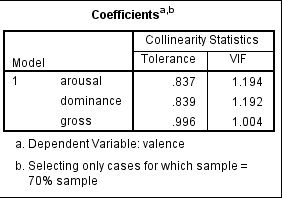
\includegraphics[width=10cm]{vif}
\end{center}

Now, observing the adjusted $R^{2}$, we can see that passing a linear curve through the scatterplot produced from 4 elements with almost no correlation produces a line of best fit with almost no relation to the actual data. In this case, our adjusted $R^{2}$-Score is 0.008, indicating no linear relationship.

\begin{center}
	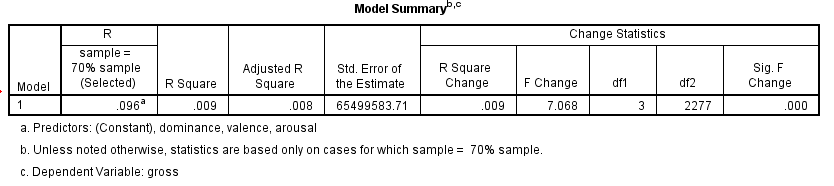
\includegraphics[width=10cm]{summary}
\end{center}

Finally, by comparing the predicted values from our training sample to a test sample, we can see that there is almost no relationship between the two, showing a pearson coefficient of ~0.
\begin{center}
	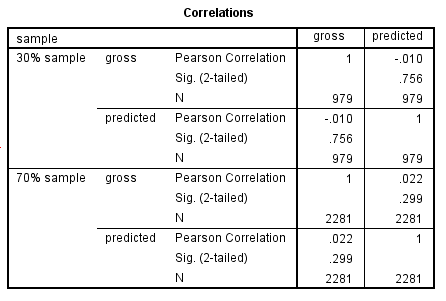
\includegraphics[width=10cm]{crossvalidation}
\end{center}

\newpage
  \section{Section 4: Conclusion}
Due to a complete lack of evidence to show any relationship between the VAD scores of a movie's title and it's corresponding box office success, we must conclude that there was insufficient evidence to support the alternative hypothesis and as a result, we retain the null hypothesis.

\textbf{The emotional impact of the lexicon used in movie titles \textit{does not have a statistically significant effect} on the box-office performance of a movie in gross revenue.}

\subsection{Discussion}
Limitations -
The dataset is quite likely too naïve to be particularly useful. The averaging method fails to account for the fact that in English, and given n-gram is likely to be more emotionally powerful than the sum of its parts, (For instance, the sentence 'For Sale: Baby's Shoes, Never Worn' tells a whole, poignant tale with very few, common words, but it would be evaluated as quite low impact in our model) but there does not currently exist a dataset that supports emotion ratings on more than unigrams, and so that is all we can use for this particularly study.
\newline \newline
Furthermore, additional factors like the value of brand recognition are not accounted for within our Dataset. A 'Spiderman' movie title would evaluate Spider and Man and provide the average for those two words, without taking into account previous connections to the name. Or in the case of "Alvin and The Chipmunks: The Squeakquel", due to the high number of nonsense words and particles, we would only evaluate the word 'Chipmunk' in the resulting average. This may have thrown off the results. In fact, movies with titles who's titles included no unigrams presented in the VAD analysis ("The Lorax" for instance), were dropped from the final set entirely. These, combined with foreign films, removed about 2000 titles from the set.
\newline \newline
Movie VAD may have an effect on a movie's box office success, but only as an additional factor to ratings and advertising budget and the like. If we were to redo this project, it may be valuable to add more explanatory factors and then attempt to isolate the effect that VAD has on the movie's success, once the majority of the model is taken up by other factors.
\newline \newline
Interestingly enough, there are some weak linear relationships present amongst the relationships between the average VAD of movie titles amongst themselves, as seen in the additional graphs appendix. This may be an area for future research, but beyond the scope of this project.






  \appendix
  \section{Additional Graphs}
\begin{center}
  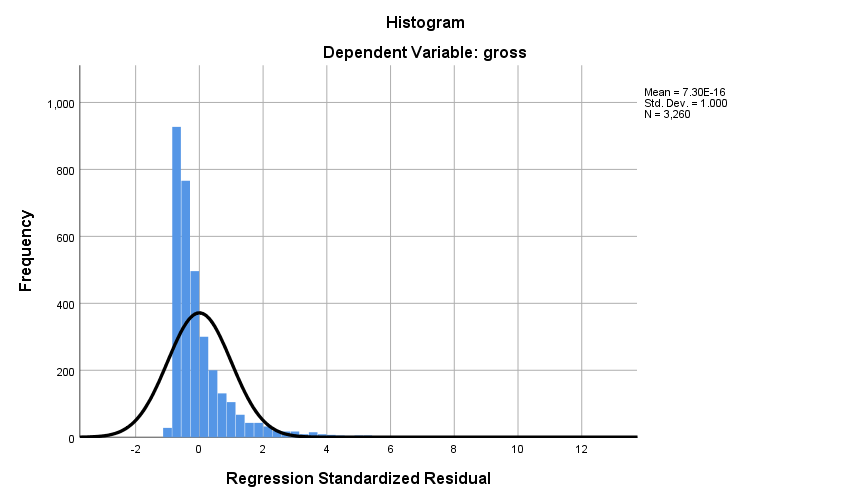
\includegraphics[width=10cm]{graph1}
\newline
  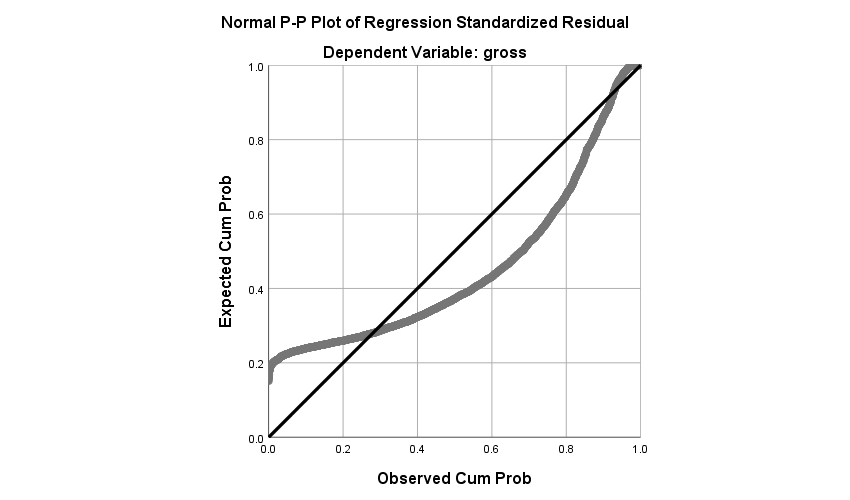
\includegraphics[width=10cm]{graph2}
\newline
  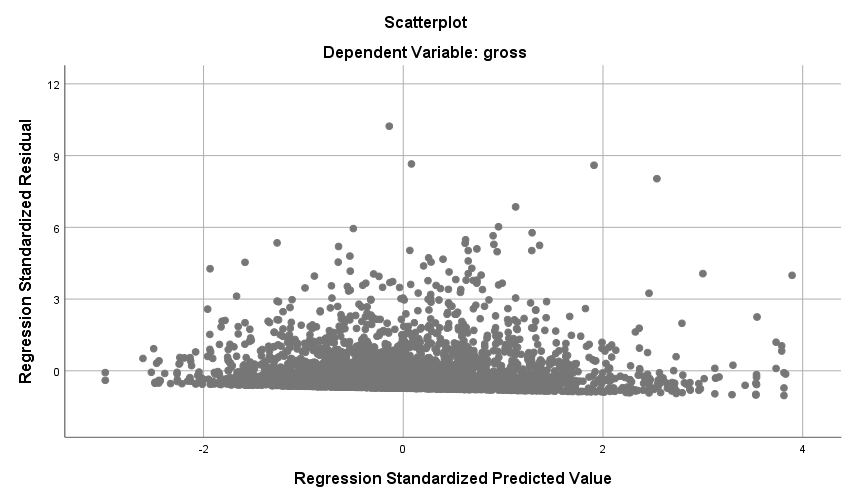
\includegraphics[width=10cm]{graph3}
\newline
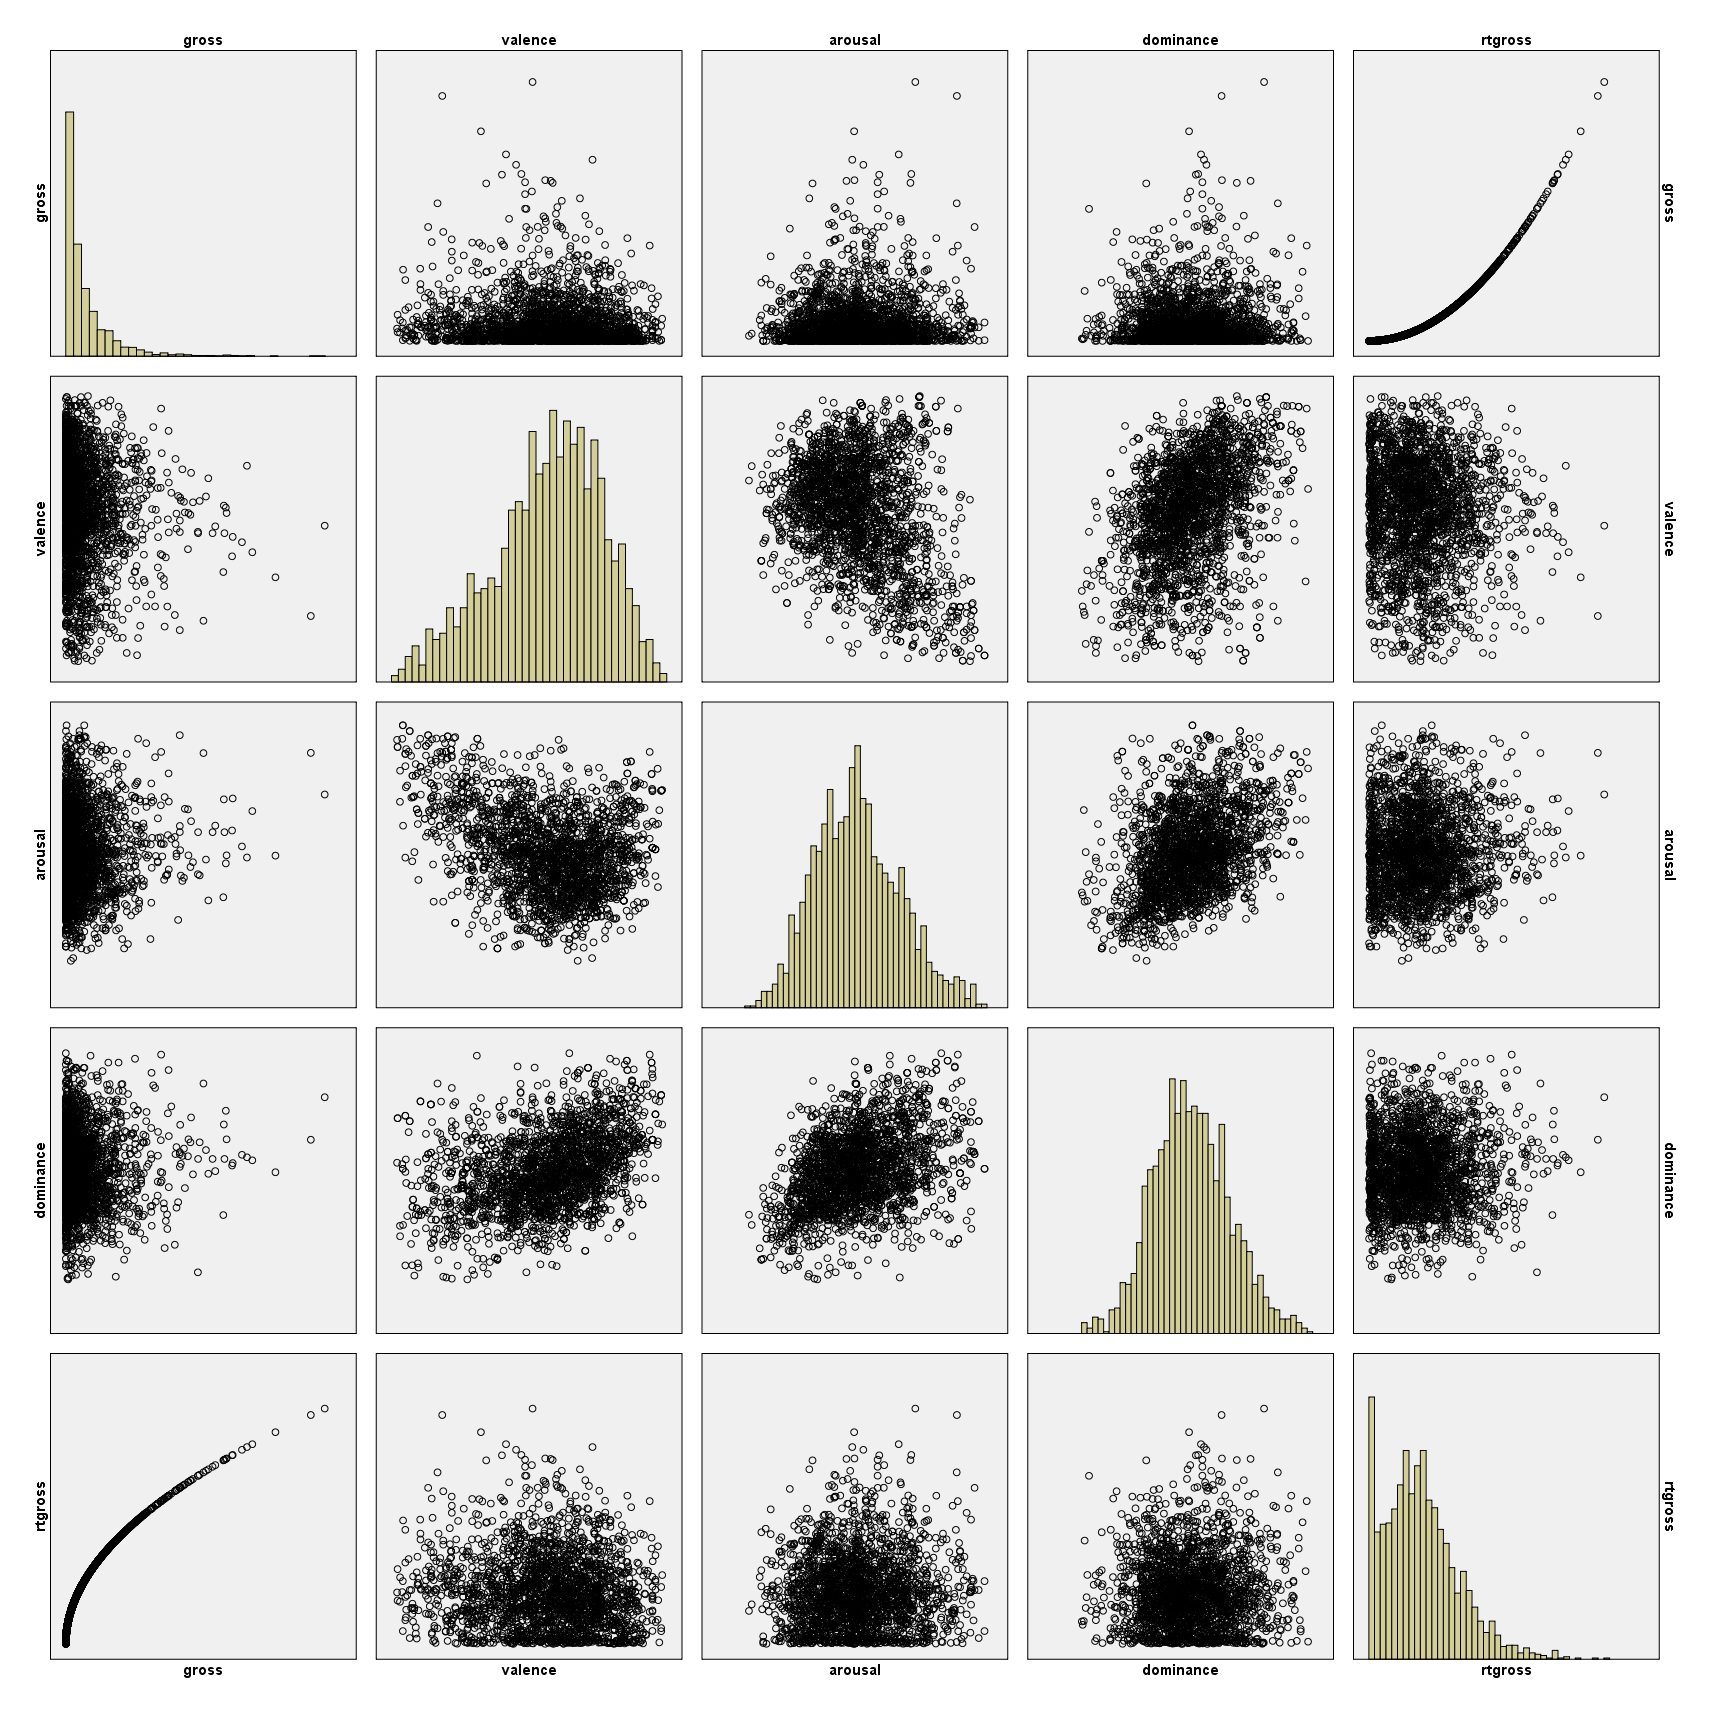
\includegraphics[width=18cm]{scatterplotmatrix}
\end{center}

\end{document}
